
%(BEGIN_QUESTION)
% Copyright 2015, Tony R. Kuphaldt, released under the Creative Commons Attribution License (v 1.0)
% This means you may do almost anything with this work of mine, so long as you give me proper credit

The most common method of starting up a three-phase induction motor is to simply apply full power all at once by closing the three contacts of a large ``contactor'' relay.  This is called {\it across-the-line} starting:

$$\includegraphics[width=15.5cm]{i02310x01.eps}$$

Across-the-line starting is simple, but results in huge ``inrush'' currents at the moment of contactor closure, and also places a lot of mechanical and thermal stress on the motor as it rushes to attain full speed.

\vskip 10pt

A ``gentler'' method of starting an induction motor is to place impedances in series with the three-phase power, using two contactors (one ``start'' and one ``run'') to sequence the motor from start-up to full-speed run.  The impedances ideally take the form of inductors (``reactors''):

$$\includegraphics[width=15.5cm]{i02310x02.eps}$$

Explain how and why this method of starting is gentler than across-the-line starting.

\vskip 20pt \vbox{\hrule \hbox{\strut \vrule{} {\bf Suggestions for Socratic discussion} \vrule} \hrule}

\begin{itemize}
\item{} Identify some means to {\it time} the closure of the two sets of power contacts (Start and Run) so that the motor is soft-started for an appropriately before having full power applied.
\item{} Would large (high-power) resistors work instead of inductors?
\item{} Would large capacitors work instead of inductors?
\item{} Suppose one of the series reactors failed open.  What effect(s) would this have on the circuit's operation?
\end{itemize}

\underbar{file i02310}
%(END_QUESTION)





%(BEGIN_ANSWER)

The ``Start'' contactor must be energized first, then at a later time is de-energized as the ``Run'' contactor is simultaneously energized.  Either timing relays or a PLC handles this sequencing of contactors.

%(END_ANSWER)





%(BEGIN_NOTES)

The reason inductors are ideal as starting impedances is because they (ideally) dissipate no power, and also help to mitigate inrush better than resistors due to their intrinsic opposite to large rates of change.  The instant of contactor switch closure tends to create very large $di \over dt$ values, which inductors work very well to minimize by creating a bucking voltage drop ($v = L {di \over dt}$).




\vskip 20pt \vbox{\hrule \hbox{\strut \vrule{} {\bf Virtual Troubleshooting} \vrule} \hrule}

This question is a good candidate for a ``Virtual Troubleshooting'' exercise.  Presenting the diagram to students, you first imagine in your own mind a particular fault in the system.  Then, you present one or more symptoms of that fault (something noticeable by an operator or other user of the system).  Students then propose various diagnostic tests to perform on this system to identify the nature and location of the fault, as though they were technicians trying to troubleshoot the problem.  Your job is to tell them what the result(s) would be for each of the proposed diagnostic tests, documenting those results where all the students can see.

During and after the exercise, it is good to ask students follow-up questions such as:

\begin{itemize}
\item{} What does the result of the last diagnostic test tell you about the fault?
\item{} Suppose the results of the last diagnostic test were different.  What then would that result tell you about the fault?
\item{} Is the last diagnostic test the best one we could do?
\item{} What would be the ideal order of tests, to diagnose the problem in as few steps as possible?
\end{itemize}

%INDEX% Final Control Elements, motor: across-the-line starting
%INDEX% Final Control Elements, motor: impedance starting

%(END_NOTES)


